\documentclass[a4paper]{article}

%% Language and font encodings
\usepackage[english]{babel}
\usepackage[utf8]{inputenc}
\usepackage[T1]{fontenc}
\usepackage[normalem]{ulem}
\usepackage{minted}
%% Sets page size and margins
\usepackage[a4paper,top=3cm,bottom=2cm,left=3cm,right=3cm,marginparwidth=1.75cm]{geometry}

%% Useful packages
\usepackage{amsmath}
\usepackage{color}
\usepackage{graphicx}
\usepackage{wrapfig}
\usepackage[colorinlistoftodos]{todonotes}
\usepackage[colorlinks=true, allcolors=blue]{hyperref}
\usepackage{listings}

\title{PHYS 370\\
Computational Physics\\}
\author{Jacob William Connelly\\
David Jedynak\\
Nick Zahler}
\date{March 07, 2018}
\begin{document}
\maketitle

\section{Abstract}
\paragraph{}
The semiconductor device is where electrical engineering meets quantum physics. By understanding the crystalline lattice structure of molecules and how charge carriers move through them, the ability to manipulate them was derived. 'Doping', the deliberate process of adding impurities into a structure, is the base theory behind the modern semiconductor. By placing two (differently) doped structures next to one another, a junction is created; this meeting of doped crystalline structures is the science behind all modern day electronics, including transistors and integrated circuits. Our experiment will seek to simulate with 3D visualizations based on C code the most basic of the semiconductor structures, the diode; a device that, when doped, only allows current to flow unidirectionally; this paper is the documentation of that experiment.

\section{Introduction}
\paragraph{}
To work through this problem we first needed to understand, in depth, the inner workings of the diode and how electricity moves through it, and why. This process was made relatively easy, since all group members have a background in electrical engineering. The trick was in figuring out how to take our knowledge of the physical chemistry of a diode, the understanding of its electrical properties, and translate that into a computer simulation. 
	The diode simulation takes the form of a plane with various fields placed along its length. For easy visualization, the different fields are denoted by lines that stretch across the plane. When the program runs with a voltage source applied in the 'proper' orientation, current will flow across the diode. However, as would happen in reality, if the voltage source is 'backwards' (or, in effect, the diode turned the other direction), current flow stops. \\
    
   

\section{Theory}
\paragraph{}
Semiconductors are unique in the electrical world in that they are able to both conduct and repel electric current. They are made of material that has an electrical conductivity between strong electric conductors, such as gold or copper, and insulators, such as rubber or plastic. The most commonly used element for semiconductor devices is silicon, a metalloid in the periodic table. Pure silicon has no free electrons, which is why the element is doped to give it enhanced electro-conductive properties. The doping process includes introducing impurities into the silicone crystal, as can be seen in Figure 1.

\begin{figure}[H]
\centering
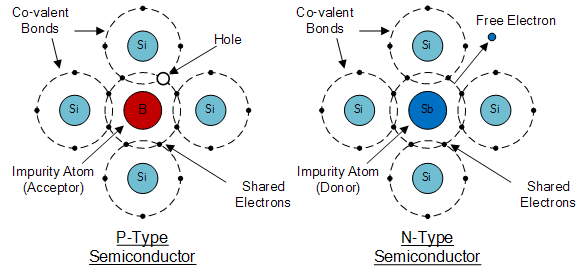
\includegraphics[scale=0.8]{doping.PNG}
\caption{\label{fig} Diagram of doping process}
\end{figure}

As noted in the figure above, N-type doping adds an impurity to the silicone structure that introduces free electrons, while P-type introduces vacant positions, or 'holes', for free electrons to fill. 

A diode is the physical object that puts this doping into practice at its most basic level. At the junction where P-type and N-type meet is where things get interesting. The extra electrons from the N-type transition over to the P-side, which gives the P-side a slightly negative charge. Simultaneously, since the electrons have moved out of the N-type region, that area gets a slightly positive charge. The electric field that results from this is known as the depletion region, which can be seen below.

\begin{figure}[H]
\centering
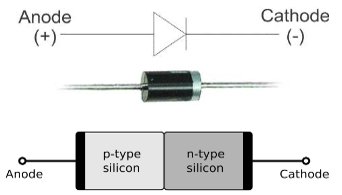
\includegraphics[scale=0.75]{Diodes2.PNG}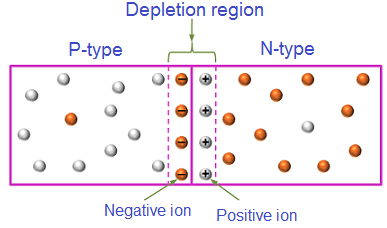
\includegraphics[scale=0.6]{Depletion.PNG}
\caption{\label{fig} Physical diode and representations (left), Depletion region (right)}
\end{figure}

The depletion region is the basis of the barrier that stops electron flow. Applying current to the diode "backwards" results in what is known as reverse biasing, in which the depletion zone widens as power source attracts both electrons and holes. However, when connected the other way, and if an electron has enough energy, it can overcome the barrier potential and cross the depletion region. Negative electrons are pushed away by negative terminal, and "fall into the holes", depleted of energy. The electrons behind it cross the barrier and occupy the next line of holes, and so on, until the holes are full, and electricity passes through the diode. This result is the one-way flow of electricity. 

In an ideal world with perfect conditions, the graph of Voltage vs Current (V vs I) should be zero at all points from negative infinity to 0V, then instantaneously spike along the y-axis at V>=0. In effect, the diode would be treated as nothing but a wire. In reality there are physical limitations on the chemical structure of silicone, which is why we need to reach a certain voltage potential before the barrier potential can be crossed. For silicone diodes, this happens at right around 0.7V. In the other direction, if a strong enough negative voltage is applied to the diode, it will eventually overpower the depletion zone and current will flow. This phenomena is known as 'breakdown', but only happens at voltages stronger than -50V, and will not be simulated in our experiment. The voltage vs current graphs of ideal vs real diodes is shown below. 

\begin{figure}[H]
\centering
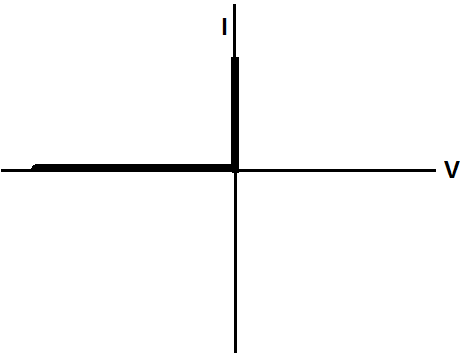
\includegraphics[scale=0.6]{08.png}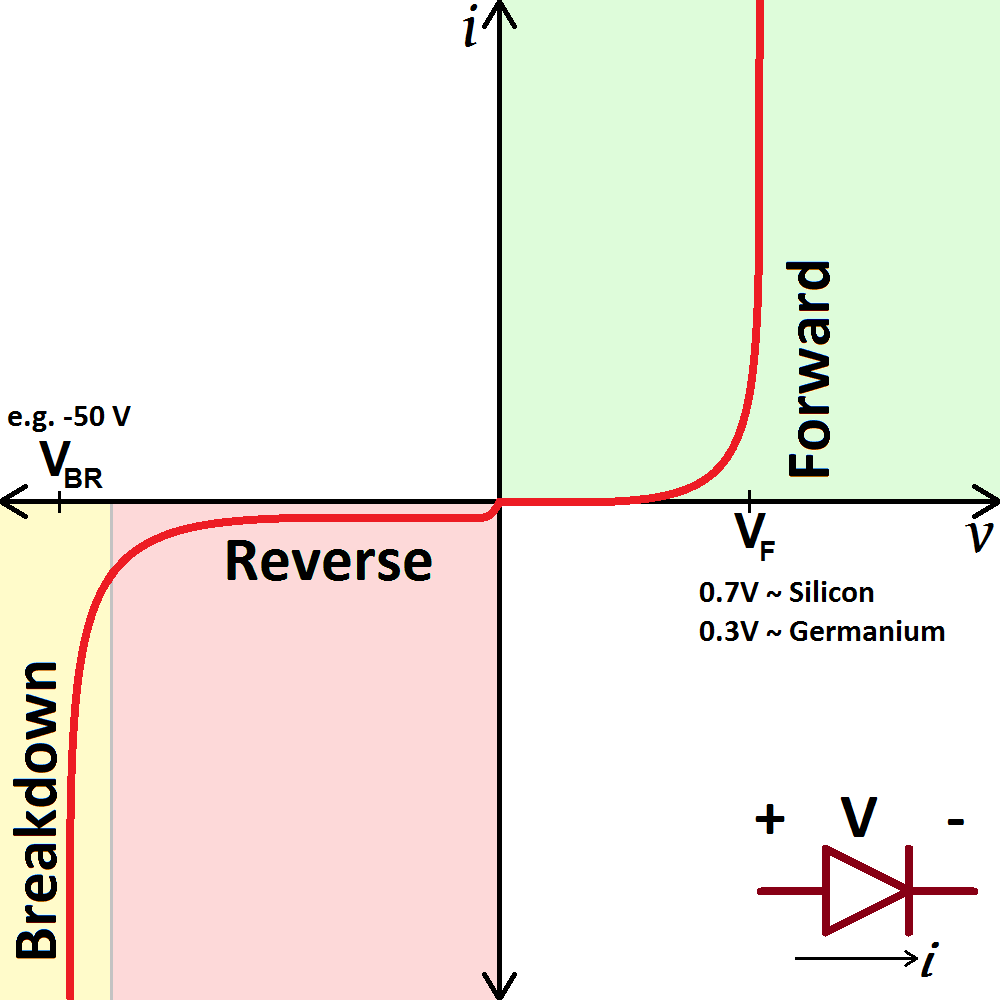
\includegraphics[scale=0.23]{06.png}
\caption{\label{fig} Ideal V vs I graph (left), Real V vs I graph (right)}
\end{figure}


\section{Simulation Design}
\paragraph{}

The general characteristics the Diode simulation is trying to model are the ability of diodes to allow current flow in one direction, the non linear relation of diode voltage and diode current, reverse bias current breakdown(i.e. exposed to a large voltage, the diode will allow reverse current), and the effect of changing the forward and reverse gap voltages. To create these behaviors, a voltage source, diode, and a resistance are needed. 

The existing simulation(MDTherm.c) from PHYS370 has most of the dynamics necessary to simulate a diode. By adding charges to the particles, they can behave similar to electrons in a circuit. To simulate the voltage source, an area in the simulation box with a vertical, horizontal, length, and width is defined. If a particle is in this "voltage" box, a force in the vertical direction is applied to move the particles and simulate electrical current. The diode is composed of 2 of these force fields(forward gap and reverse gap) that are similar to the voltage source, but the forward gap only acts on particles moving with positive vertical velocity, and the downward gap acts on those with negative vertical velocity.

\subsection{Theory-Mathematics}

We need to be able to set voltages using force. Using the equations below a relation between force and voltage can be derived.

Where E ~ Electric Field, V ~ Voltage, Q ~ particle charge, dl ~ Field Length

$ V = \vec{E}*dl $ 
$ \vec{E} = \frac{\vec{N}}{Q} $

Derived relation between Voltage and Force:

$ \vec{N} = \frac{V*Q}{dl}$

Similarly this can done for resistance:

\subsubsection{Requirements}

Inputs
\begin{enumerate}
\item Voltage Source (Voltage)
\item Particle Charge
\item Forward Diode Gap (Voltage)
\item Reverse Diode Gap (Voltage)
\item Voltage Sweep ~ v start, v end, increment voltage, averaging time
\end{enumerate}

Outputs
\begin{enumerate}
\item .dat file with the VI Curve for analysis
\item Real time current graph
\item graphics lines on the simulation to notate circuit components
\end{enumerate}

\subsection{Code Explained}
\paragraph{Subroutines}

This subroutine calculates the average current by summing the voltages, dividing by box length (L) and multiplying by particle charge.

\begin{minted}{c}
// functions defined for midterm
double getCurrent(double v[N][D]){
	double sumV = 0;
	for(int n = 0;n<N;n++){
		sumV += v[n][1];
		}
	return iq*sumV/L;
}
\end{minted}

This subroutine calculates the forces for the different components based on the input voltages, resistances. It also sets the charge of the particles. This makes it easier to change parameters quickly while simulating

\begin{minted}{c}
void setVoltageSource(){
  //calculate forces for the given voltages
  v_f = iq*vs_v/volt_len;		//calculate the field from the set voltage
  ud_f = iq*ud_v/diode_len_p;		//calculate the field from the set upper diode voltage gap
  dd_f = iq*dd_v/diode_len_n;		//calculate the field from the lower diode votlage gap
  for (int n=0; n<N; n++){
    for (int d=0; d<D; d++){
    q[n] = iq;				//set initial charge for each electron
    }}

}
\end{minted}

This routine sweeps the voltage from start to end with an increment, outputs a file with the voltage and current information to look at diode VI characteristics.

\begin{minted}{c}
void VI_Curve(){
  FILE *res;
  char IsoName[100];
  double sumI = 0;

  sprintf(IsoName,"VI_Curve_Q_%f_N_%i_ud_v_%f_dd_v_%f.dat",iq,N,ud_v,dd_v);//put info in the filename to distinguish test params
  res=fopen(IsoName,"w");
  //sweep the voltage
  if(v_incr < 0 ){
	  for (double ivolt = v_start;ivolt>v_end;ivolt = ivolt + v_incr){
		//set the voltage
		vs_v = ivolt;
		setVoltageSource();
		//loop to waste some time to get the current to settle
		for(int t = 0;t<v_sweep_delta;t++)
			{
			iterate(x,v,dt);
	       	 	Events(1);
			DrawGraphs();
			sumI += current_var;
			}
		//save the current and voltage data
		fprintf(res,"%e %f\n",sumI/v_sweep_delta,vs_v);
	   }
   }
     else{
	  for (double ivolt = v_start;ivolt<v_end;ivolt = ivolt + v_incr){
		//set the voltage
		vs_v = ivolt;
		setVoltageSource();
		//loop to waste some time to get the current to settle
		for(int t = 0;t<v_sweep_delta;t++)
			{
			iterate(x,v,dt);
	       	 	Events(1);
			DrawGraphs();
			sumI += current_var;
			}
		//save the current and voltage data
		fprintf(res,"%e %f\n",sumI/v_sweep_delta,vs_v);
	   }
   }

  fclose(res);
}

\end{minted}

Code added to draw() subroutine to draw lines where the voltage source, diode, and resistor fields exist.

\begin{minted}{c}

//voltage source lines
  mydrawline(2,0,scalefac*(L-volt_pos+volt_len/2),size,scalefac*(L-volt_pos+volt_len/2));
  mydrawline(2,0,scalefac*(L-volt_pos-volt_len/2),size,scalefac*(L-volt_pos-volt_len/2));

//diode field 1 lines
  mydrawline(3,0,scalefac*(L-diode_pos_p + diode_len_p/2),size,scalefac*(L-diode_pos_p + diode_len_p/2));
  mydrawline(3,0,scalefac*(L-diode_pos_p - diode_len_p/2),size,scalefac*(L-diode_pos_p - diode_len_p/2));

//diode field 2 lines
 // mydrawline(4,0,100,size,100);
  mydrawline(4,0,scalefac*(L-diode_pos_n - diode_len_n/2),size,scalefac*(L-diode_pos_n - diode_len_n/2));

//resistor field lines
  mydrawline(6,0,scalefac*(L-res_pos+res_len/2),size,scalefac*(L-res_pos+res_len/2));
  mydrawline(6,0,scalefac*(L-res_pos-res_len/2),size,scalefac*(L-res_pos-res_len/2));

\end{minted}

\paragraph{Code added to iterate routine}

This code iterates through each particle and determines a force to apply to each particle depending on their position and velocity. This simulates the voltage source, diode, and a resistor(the resistor is untested).

\begin{minted}{c}
    for (int n=0;n<N;n++)
      for (int d=0;d<D;d++){
	//begin conditions for diode, resistor, and voltage source regions
	v[n][d]+=(ff[n][d])/mass[n]*dt;// integrate to get velocity
	
	if (d == 1){// if the dimension is in the Y dimension... vertical
	//check to see if the particle is in diode p, diode n, voltage, resistor regions, then apply the appropriate force
		if ((x[n][d] < (diode_pos_p+diode_len_p/2)) && (x[n][d] > (diode_pos_p-diode_len_p/2))&& v[n][d] < 0){//upward diode field.. if the particle has -v then force particle upwards
			field_force = ud_f - current_var;//simulate the forward diode band gap
			}
		else if((x[n][d] < (diode_pos_n+diode_len_n/2)) && (x[n][d] > (diode_pos_n-diode_len_n/2))&& (v[n][d] > 0)){//downward diode field... stops reverse bias current throgh the diode
			field_force = dd_f + current_var;//simulate the reverse diode band gap
			}
		else if((x[n][d] < (volt_pos + volt_len/2)) && (x[n][d] > (volt_pos - volt_len/2))){//voltage source field... provides electromotive force to propel particles throgh diode
			field_force = v_f;//simualate voltage source
			}
		else if((x[n][d] > (res_pos - res_len/2)) && (x[n][d] < (res_pos + res_len/2)) && abs(v[n][d]) > 0){//resistor field... just a resistor for fun
			field_force = -v[n][d]*q[n]*q[n]*resistance/(res_len*res_len);// derived from V=IR, V=E*dl, E=N/C
			}
		else{
			field_force = 0;	//particle is not in a component, then no force.	
		}
	v[n][d]+=(field_force)/mass[n]*dt;//integrate again to update velocity with the accelerations of the fields
	
	}
	else{
		field_force = 0;		
		}

	}
\end{minted}



\paragraph{Code added for graphing data}

Observing how current changes when different inputs changed was important to verify that the program was functioning properly.

Storing current data
\begin{minted}{c}
  //storing current values for graphing later
  memmove(&IImeas[1],&IImeas[0],(MeasMax-1)*sizeof(double));
  IImeas[0]=current_var;
\end{minted}

Plotting current data with respect to time
\begin{minted}{c}
DefineGraphN_R("Average Current",&IImeas[0],&Measlen,NULL);
\end{minted}

\begin{figure}[H]
\centering
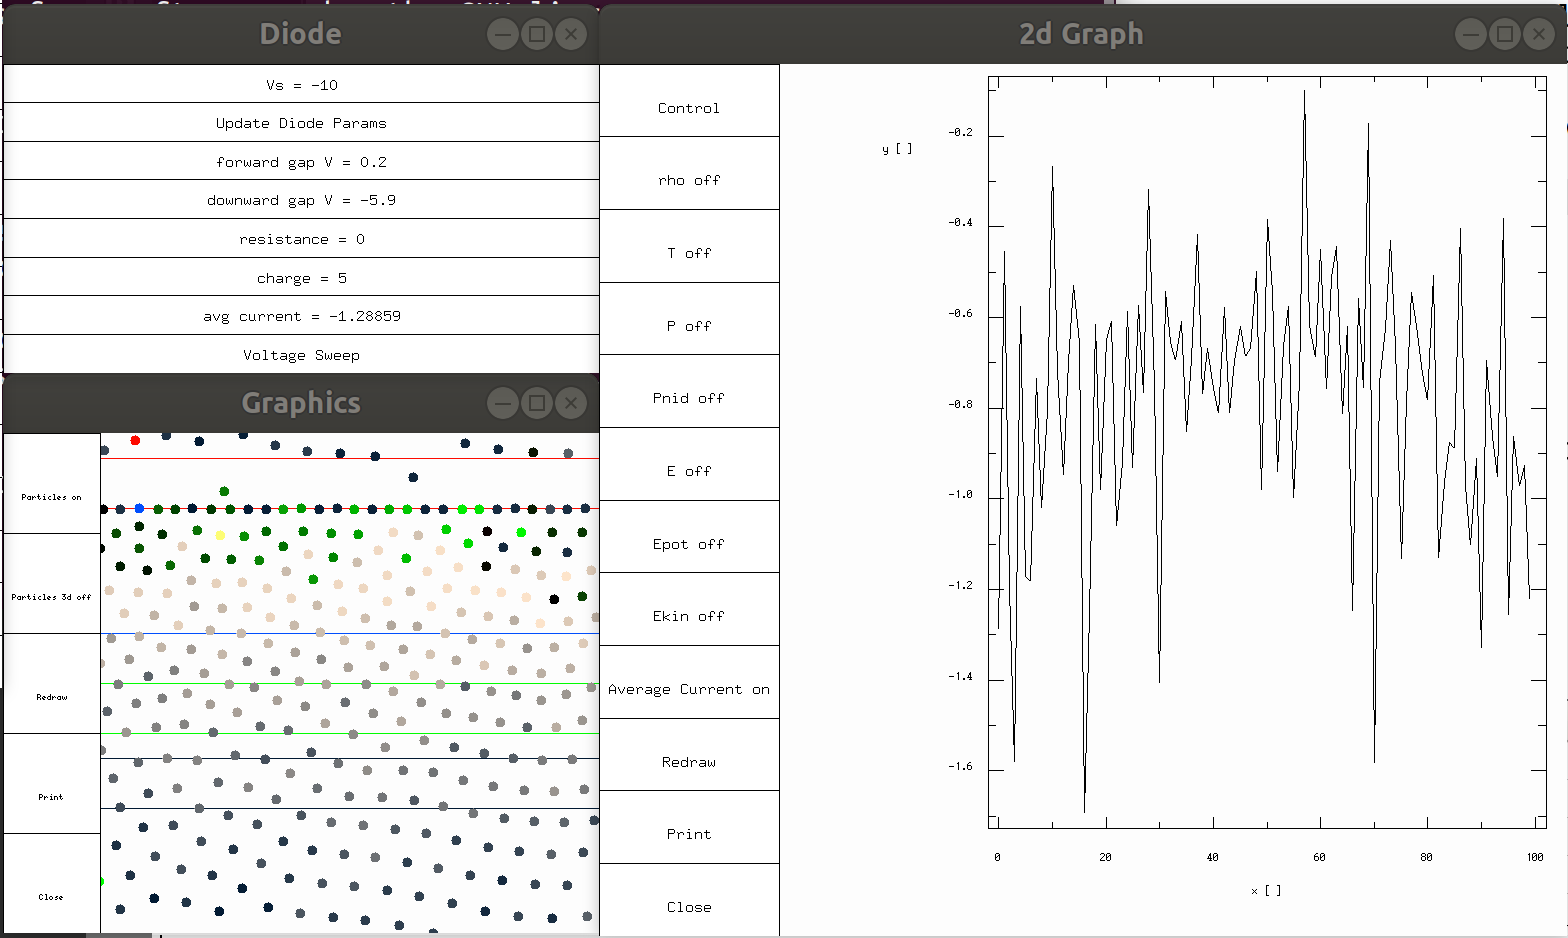
\includegraphics[scale=0.2]{current_graph.png}
\caption{\label{fig} plot of the diode current vs time}
\end{figure}



\paragraph{Code added to GUI for running diode simulation}
\begin{minted}{c}
  //menu code for diode midterm
  StartMenu("Diode",0);
  DefineDouble("Vs",&vs_v);
  DefineFunction("Update Diode Params",setVoltageSource);
  DefineDouble("forward gap V",&ud_v);
  DefineDouble("downward gap V",&dd_v);
  DefineDouble("resistance",&resistance);
  DefineDouble("charge",&iq);
  DefineDouble("avg current",&current_var);
  StartMenu("Voltage Sweep",0);
  DefineFunction("VI Curve",VI_Curve);
  DefineDouble("V start",&v_start);
  DefineDouble("V end",&v_end);
  DefineDouble("v_incr",&v_incr);
  DefineInt("v_sweep_delta",&v_sweep_delta);
  EndMenu();
\end{minted}




\section{Procedure}
\paragraph{}
\begin{enumerate}
\item Open terminal and launch the Diode program with the following command
\begin{minted}{bash}
  $./diodeexec$
\end{minted}
\item Click init, measure, Measurements and Diode. All of these should bring up a separate window. Arrange these on your desktop so you can see all of them.
\item leave other settings set to defaults
\item in the Measurements window, click Average Current to open a line graph of current over time. This should have a dynamic graph once cont is set to on.
\item In the Diode window, click Update Voltage Params to initialize the voltage.
\item in the main window, set cont to on
\item Click graph to see the simulation itself run
\item To run a voltage sweep and collect data of V vs I, click Diode > Voltage Sweep. This will open another window.
\item Set V start and V end to desired parameters.
\item Click VI Curve to run the voltage sweep.
\item *Note: To adjust the initial forward gap voltage of the diode, change the parameters in Diode > forward gap V. It defaults to 0.2
\end{enumerate}

\section{Results}
\paragraph{}

\begin{figure}[H]
\centering
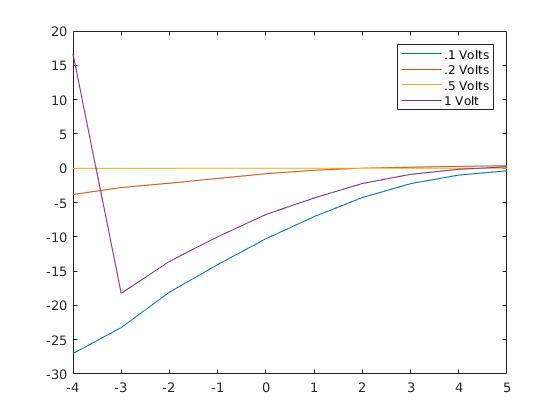
\includegraphics[scale=0.5]{vi_curves.jpg}
\caption{\label{fig} plot of several vi curves with different forward diode voltages, we expected the curves to slope faster with lower diode voltage, but this wasn't always observed}
\end{figure}

\begin{figure}[H]
\centering
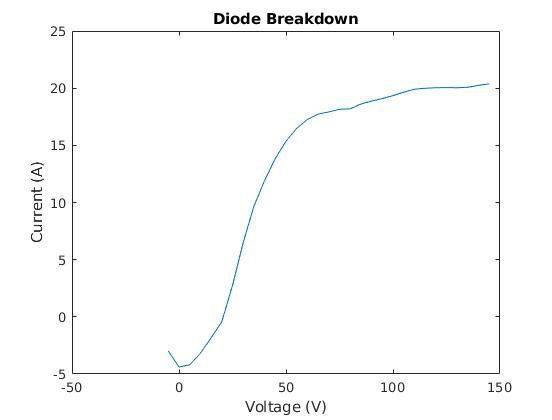
\includegraphics[scale=0.5]{diode_break.jpg}
\caption{\label{fig} plot of several vi curves with different forward diode voltages}
\end{figure}

\begin{figure}[H]
\centering
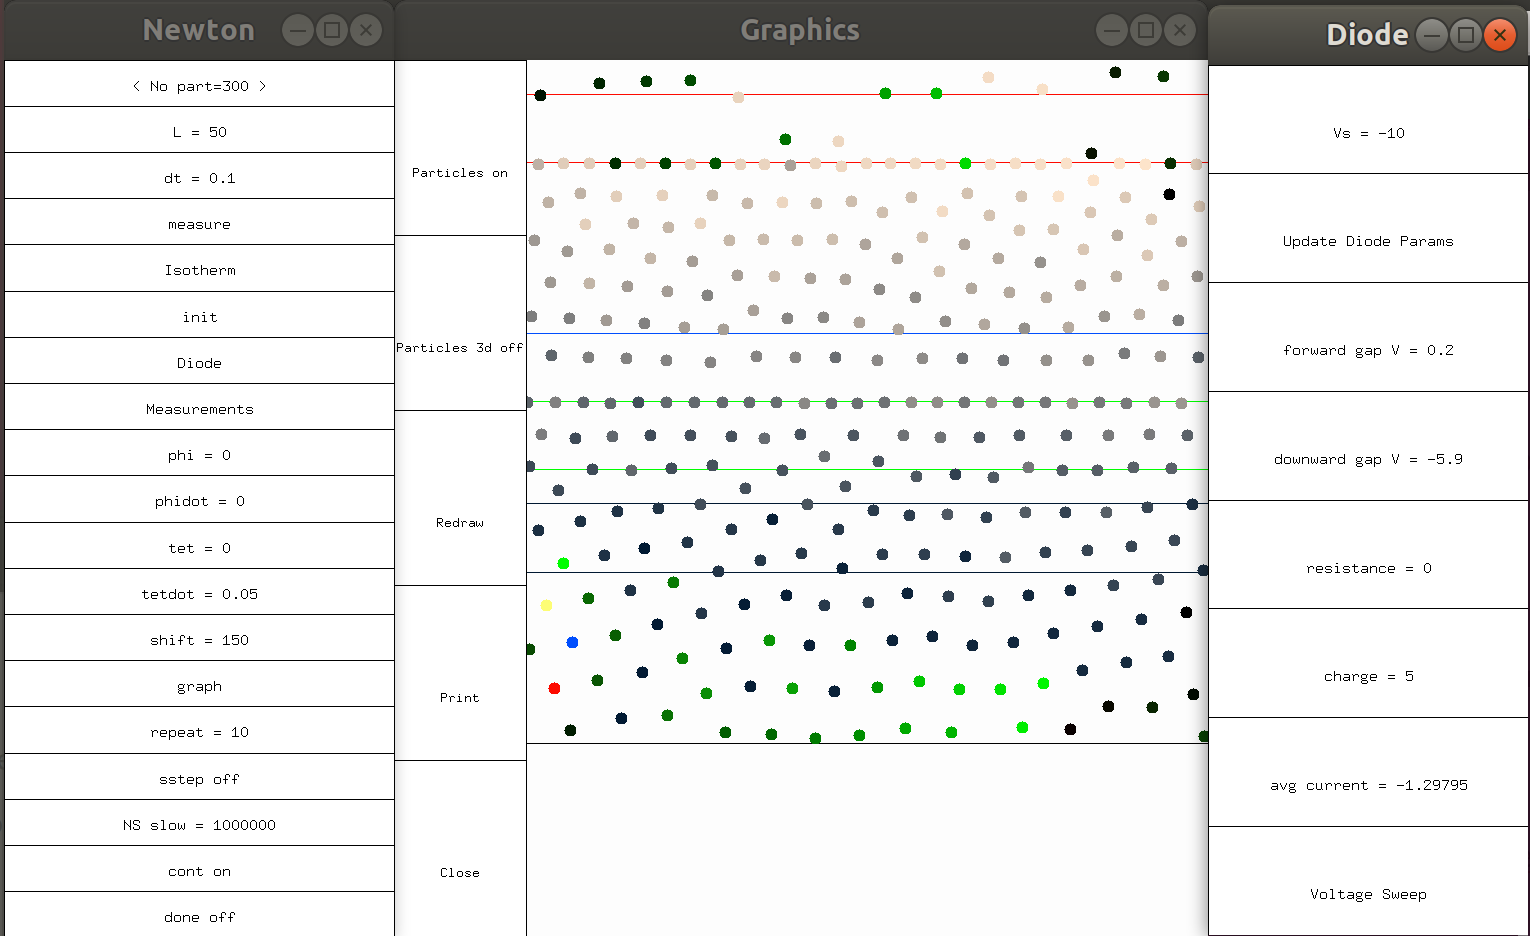
\includegraphics[scale=0.3]{sim.png}
\caption{\label{fig} Photograph of the simulation running, Red lines mark voltage source, blue is reverse diode field and green is forward diode field}
\end{figure}


\section{Conclusion}
\paragraph{}
Over the course of the project, the group ran into many logic errors in the c code. In order to find these problems we added print statements, and eventually we started using a debugger. We did resolve these errors allowing us to complete the simulation code. The logic errors in the code originally caused the diode conditions not to work because the velocities of all the particles were zero. This caused issues because our Diode logic relied on know which direction the particles were heading. This issue was resolved by changing the order of the code in iterate so the velocities were computed before the diode code was executed. We also observed particles traveling very quickly. This could be due to an integration error. We were able to observe typical silicone diode Voltage Current Curves, however they were very linear for the forward and the reverse breakdown current section. The whole voltage current curve was non linear in that the diode does stop small reverse currents, but allows forward currents.

\section{Individual Contribution}
\paragraph{}
 The group had a wide variety of skill levels in different domains. The goal was to select tasks that each member could realistically complete while giving each person something challenging that they could learn from. We all used a mobile phone group chat to stay in contact.
 
Jacob Connelly:Throughout the lifespan of this project, Jacob's main contribution was in the writing of the LaTeX document and background research on diode theory, including crystalline structure, the concept behind forward and reverse bias, and the points at which the diode behaves either as expected (under normal conditions) or breaks (under less ideal conditions). He was also responsible for running the simulations under test conditions to collect results.

David Jedynak focused on writing the diode code logic, plotting code, simulation design, and writing the simulation design subsection in the latex paper. Also he showed his group members how to use an online code repository(Github).

Nick Zahler:For the midterm, I helped David develop the region idea for the “force field” that we used in the program. We both tried to make it with our own way, and in the end decided to use David’s version of the code due to it behaving more consistently than my version. I also helped get the LaTex document in order for submission, and gathered the data from Jacob for the graphs of the VI curves and the diode breakdown. Once I had the data, I used Matlab to generate graphs that we include in our submission.  Using Matlab also helped us spot unusual behavior that we had with any of the simulations. Also, I reviewed the code being written and assisted David whenever he needed debugging. I also tried to get a resistance sweep function to work, however ran into lots of problems, and for the sake of compiling our code, we got rid of it. I attempted to smooth out some of the early renditions of the VI Curves code due to low voltage results having erratic behavior. In the end, we re-did some of the math and rearranged the code for it to run a little bit smoother. Overall, my group partners did superb in helping the group achieve their goal. 


\section{Code for Diode Simulation}
\paragraph{}

\lstinputlisting[language=C]{/home/david/Documents/Computational_Physics/Midterm_Diode/diode.c}

\section{References}
\paragraph{}
https://www.ndsu.edu/pubweb/~carswagn/LectureNotes/370/index.html

\begin{lstlisting}
Figure 1: \\http://www.expertsmind.com/learning/p-type-semiconductor-basics-assignment-help-7342873147.aspx\\
Figure 2 (left): \\https://www.electrical4u.com/diode-working-principle-and-types-of-diode/\\
Figure 2 (right): \\http://www.electricalworld360.com/depletion-region/\\
Figure 3 (left): \\http://www.learningaboutelectronics.com/Articles/Ideal-diode.php\\
Figure 3 (right):\\https://learn.sparkfun.com/tutorials/diodes/real-diode-
\end{lstlisting}


\end{document}



++++++++++++

